% This file was created with tikzplotlib v0.10.1.
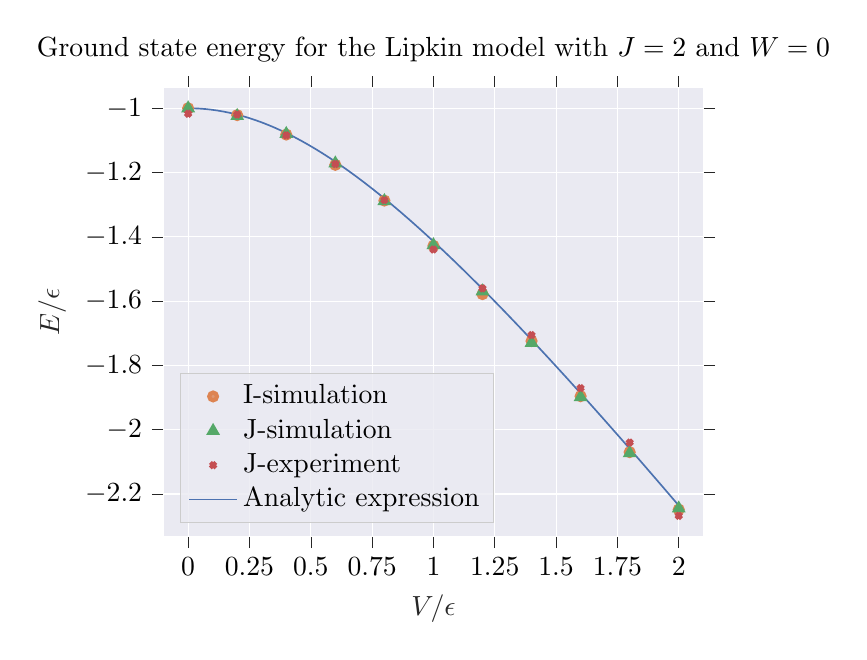
\begin{tikzpicture}

\definecolor{darkslategray38}{RGB}{38,38,38}
\definecolor{indianred1967882}{RGB}{196,78,82}
\definecolor{lavender234234242}{RGB}{234,234,242}
\definecolor{lightgray204}{RGB}{204,204,204}
\definecolor{mediumseagreen85168104}{RGB}{85,168,104}
\definecolor{peru22113282}{RGB}{221,132,82}
\definecolor{steelblue76114176}{RGB}{76,114,176}

\begin{axis}[
axis background/.style={fill=lavender234234242},
axis line style={white},
legend cell align={left},
legend style={
  fill opacity=0.8,
  draw opacity=1,
  text opacity=1,
  at={(0.03,0.03)},
  anchor=south west,
  draw=lightgray204,
  fill=lavender234234242
},
mark options={mark size=1.4pt, line width=1.5pt},
minor xtick={},
minor ytick={},
tick align=outside,
title style={align=center},
title={Ground state energy for the Lipkin model with \(\displaystyle J = 2\) and \(\displaystyle W = 0\)},
x grid style={white},
xlabel=\textcolor{darkslategray38}{\(\displaystyle V/\epsilon\)},
xmajorgrids,
xmajorticks=false,
xmajorticks=true,
xmin=-0.1, xmax=2.1,
xtick style={color=darkslategray38},
xtick={-0.25,0,0.25,0.5,0.75,1,1.25,1.5,1.75,2,2.25},
y grid style={white},
ylabel=\textcolor{darkslategray38}{\(\displaystyle E/\epsilon\)},
ymajorgrids,
ymajorticks=false,
ymajorticks=true,
ymin=-2.3314697265625, ymax=-0.9365966796875,
ytick style={color=darkslategray38},
ytick={-2.4,-2.2,-2,-1.8,-1.6,-1.4,-1.2,-1,-0.8}
]
\addplot [draw=peru22113282, fill=peru22113282, mark=*, only marks]
table{%
x  y
0 -1
0.2 -1.02142
0.4 -1.08188
0.6 -1.17602
0.8 -1.28728
1 -1.4281
1.2 -1.57824
1.4 -1.7242
1.6 -1.89588
1.8 -2.06996
2 -2.2485
};
\addlegendentry{I-simulation}
\addplot [draw=mediumseagreen85168104, fill=mediumseagreen85168104, mark=triangle*, only marks]
table{%
x  y
0 -1
0.2 -1.02406
0.4 -1.07984
0.6 -1.1713
0.8 -1.28864
1 -1.4257
1.2 -1.56956
1.4 -1.72966
1.6 -1.8985
1.8 -2.07328
2 -2.2449
};
\addlegendentry{J-simulation}
\addplot [draw=indianred1967882, fill=indianred1967882, mark=x, only marks]
table{%
x  y
0 -1.01689453125
0.2 -1.01962890625
0.4 -1.0841796875
0.6 -1.1734375
0.8 -1.28583984375
1 -1.439453125
1.2 -1.56044921875
1.4 -1.70576171875
1.6 -1.870703125
1.8 -2.040234375
2 -2.26806640625
};
\addlegendentry{J-experiment}
\addplot [semithick, steelblue76114176]
table {%
0 -1
0.0240000486373901 -1.00028800964355
0.0479999780654907 -1.00115132331848
0.0720000267028809 -1.0025886297226
0.0959999561309814 -1.00459742546082
0.120000004768372 -1.00717425346375
0.144999980926514 -1.01045787334442
0.169999957084656 -1.01434707641602
0.194999933242798 -1.01883506774902
0.220000028610229 -1.02391409873962
0.245000004768372 -1.02957510948181
0.271000027656555 -1.03606998920441
0.296999931335449 -1.04317259788513
0.322999954223633 -1.05087053775787
0.350000023841858 -1.05948102474213
0.376999974250793 -1.06870436668396
0.404999971389771 -1.07889986038208
0.432999968528748 -1.08971965312958
0.462000012397766 -1.10156428813934
0.490999937057495 -1.11403810977936
0.521000027656555 -1.12758195400238
0.552000045776367 -1.14223635196686
0.58299994468689 -1.15753579139709
0.615000009536743 -1.17397832870483
0.648000001907349 -1.19159722328186
0.681999921798706 -1.21042311191559
0.716000080108643 -1.22990083694458
0.751999974250793 -1.25120103359222
0.789000034332275 -1.27378213405609
0.827000021934509 -1.29766285419464
0.865999937057495 -1.32285904884338
0.906000018119812 -1.34938359260559
0.947999954223633 -1.37793469429016
0.991999983787537 -1.40856802463531
1.03699994087219 -1.44061410427094
1.08399999141693 -1.47480714321136
1.13300001621246 -1.51118791103363
1.18400001525879 -1.54979228973389
1.23699998855591 -1.59065043926239
1.29200005531311 -1.63378822803497
1.35000002384186 -1.6800297498703
1.41100001335144 -1.72942793369293
1.47500002384186 -1.78202831745148
1.54200005531311 -1.83786940574646
1.61199998855591 -1.8969829082489
1.68499994277954 -1.95939409732819
1.76199996471405 -2.02599215507507
1.84300005435944 -2.09681868553162
1.92999994754791 -2.17368340492249
1.99899995326996 -2.23517370223999
};
\addlegendentry{Analytic expression}
\end{axis}

\end{tikzpicture}
